\section{Bayesian Filtering}
\subsection{Overview}

This chapter introduces and describes the Bayesian approach for solving inverse problems, laying out the theoretical foundations of the taken approach. In Section 2.2 we present the class of problems we will be considering in this thesis: finite-dimensional inverse and filtering problems. In Section 2.3 we present a filtering problem based on a simple dynamical system estimation problem which will be used to illustrate concepts presented throughout the thesis. In Section 2.4 we define desired characteristics of solutions to inverse problems. We mention the challenges encountered by the classical optimization approach for solving inverse problems in practical situations. We then present the Bayesian framework, and show how it uses prior information about the structure of the problem to construct a solution to the inverse and filtering problems. In Section 2.5 we prove well-posedness of this constructed solution under some light assumptions about the model. Finally, Section 2.6 illustrates Bayesian modelling by describing the process of constructing a probabilistic model for the pendulum problem, and show that the problem is well-posed and thus admits a stable solution.

\subsection{Set-Up}

We study parametrized models for which the value of the \textit{parameter} $u \in X$ is unknown or uncertain. To model the behaviour of the system, we introduce \textit{forward response operators} $\mathcal{G} : X \rightarrow Y$ mapping values of the \textit{parameter space} to the \textit{data space}, assuming both spaces to be finite-dimensional vector spaces.

We consider a real system described by $\mathcal{G}$ and the true parameter $u^* \in X$, and assume that \textit{observations} $y^{obs} \in Y$ of the system are available from measurements. The data $y$ is then the image of the true parameter under the mapping $\mathcal{G}$. Due to noise present in the data, we obtain the following approximate model

\begin{equation}\label{inverse-formula}
  y^{obs} \approx \G(u^*),
\end{equation}

and the question \textit{To which extent can we find the \textit{inverse} of the data $y^{obs}$ under the forward response operator $\G$?} Answering this question is known as the \textit{inverse problem}.

In this thesis, we are interested in solving the inverse problem by incrementaly building up knowledge about the unknown parameter $u^*$. To do this, we decompose the data and consider a growing sequence of observations made available for analysis. The advantages of this approach are twofold. First, it allows to perform inference on running dynamical systems and update our knowledge as more measurements become available. Second, it can also be used in situations where all the data is available to transform one large problem in a sequence of smaller problems that can hopefully be solved more efficiently.

In this sequential formulation, the data $y$ is decomposed in a finite sequence of observations $y^{obs} = (y^{obs}_1, \ldots, y^{obs}_T)'$ \note{maybe it's relevant to cite \cite{chopin_2002} here}. We also decompose the forward response operator $\G$ in a sequence of operators $\G_1, \ldots, \G_T$ such that

\begin{equation*}
  y^{obs}_t\approx \G_t(u^*).
\end{equation*}


This allows us to reformulate the question from above as \textit{How can we use new observations to update our knowledge about $u^*$?} Answering this new question is called the \textit{filtering problem}. This thesis will focus on solving inverse and filtering problems.

One situation where this decomposition can naturally be used is when the system is described by an initial value problem of the form

\begin{equation}
  \begin{aligned}
    \frac{\text{d}x}{\text{d}t} &= f(x; u^*)\\
    x(0) &= x_0,
  \end{aligned}
\end{equation}  

where $u^* \in X$ is the parameter of the model, and the solution $x(t; u^*)$ is assumed to exist for every time $t \geq 0$. The sequence of observations then correspond to measurements at times  $0 \leq t_1 < \ldots < t_T$. We further use an \textit{observational operator} $\mathcal{O}$ to model the measurement procedure, mapping states of the system to observations. The forward response operators are then given by $\G_i = \mathcal{O} \circ x(t_i; \cdot)$ for $i = 1, \ldots, T$. We provide an example of the modelling of a inverse problem in the next section.

\subsection{Pendulum problem}

We now introduce a filtering problem that will guide the rest of the thesis. Using a pendulum, we would like to estimate the value of the Earth's gravitational acceleration. We start by modelling the behaviour of the pendulum using a differential equation parametrized by the gravitational acceleration $g$.

We choose the \textit{simple pendulum model}, a simplified mathematical model that ignores the mass of the string of the pendulum and ignores the forces of friction acting on the hanging mass. It also assumes that the movement of the pendulum only happens in two dimensions. This simplification allows us to model the state of the pendulum with a single value $x(t)$ representing the angle of the pendulum to the resting point, described by the following second order differential equation.

\begin{equation}\label{pendulum-ode}
  \frac{\text{d}^2x}{\text{d}t^2} = -\frac{g}{l}\sin(x).
\end{equation}

In this model, $g$ is the Earth's gravitational acceleration and $l$ is the length of the string holding the hanging mass. Figure \ref{pendulum-fig} represents the pendulum in this model, the vertical vector represents the gravitational force and the red and blue vectors represent the same force decomposed into its components, parallel and perpendicular to the motion of the pendulum.


We then ran an experiment in which the pendulum was let go from an initial angle of $5^\circ$ and no initial velocity. Using a stopwatch, we collected $T=11$ time measurements at which the pendulum was aligned with the vertical axis, corresponding to a null angle of the pendulum.

\begin{figure}\label{pendulum-fig}
  \centering
  \begin{tikzpicture}
    % save length of g-vector and theta to macros
    \pgfmathsetmacro{\Gvec}{1.5}
    \pgfmathsetmacro{\myAngle}{30}
    % calculate lengths of vector components
    \pgfmathsetmacro{\Gcos}{\Gvec*cos(\myAngle)}
    \pgfmathsetmacro{\Gsin}{\Gvec*sin(\myAngle)}

    \coordinate (centro) at (0,0);
    \draw[dashed,gray,-] (centro) -- ++ (0,-2.9) node (mary) [black,below]{$ $};
    \draw[dashed,gray,-] (0,-3.5) -- ++ (0,-0.5);
    \draw[thick] (centro) -- ++(270+\myAngle:3) coordinate (bob)
      node[near end,above right] {$l$};
    \pic [draw, -, "$x$", angle eccentricity=1.5] {angle = mary--centro--bob};
    \draw [red,-stealth] (bob) -- ($(bob)!-\Gcos cm!(centro)$)
      coordinate (gcos)
      node[near end, right] {$mgl\cos x$};
    \draw [blue,-stealth] (bob) -- ($(bob)!\Gsin cm!90:(centro)$)
      coordinate (gsin)
      node[near end,below left] {$mgl\sin x$};
    \draw [-stealth] (bob) -- ++(0,-\Gvec)
      coordinate (g)
      node[below] {$mgl$};
    \filldraw [fill=black!40,draw=black] (bob) circle[radius=0.1];
\end{tikzpicture}


%%% Local Variables:
%%% mode: latex
%%% TeX-master: "Thesis"
%%% End:

  \caption{Pendulum model and forces applied to the mass.   }
\end{figure}

\subsection{Bayesian filtering}

The previous sections defined the inverse and filtering problems. Before starting to discuss solutions to these problems, we present the concept of \textit{well-posedness} first given by Hadamard in \cite{hadamard} for describing properties of models of physical phenomena.

\begin{definition} A problem is said to be \textit{well-posed} if it satisfies the following conditions:
  \begin{enumerate}
  \item{a solution exists,}
  \item{the solution is unique,}
  \item{the solution changes continuously with respect to the initial condition.}
  \end{enumerate}

  A problem failing to satisfy these conditions is said to be \textit{ill-posed}. In the context of inverse problems, the third property states that small perturbations in the data should result in proportionally small perturbations in the solution $u$ of the inverse problem.  
\end{definition}

A possible way to solve inverse problems is to try to find a value $\hat u \in X$ that solves the inverse problem \textit{as well as possible}. This is done by replacing the inverse problem by the following optimization problem

\begin{equation*}
  \hat u = \underset{u \in X}{\text{argmin}} \norm{ y^{obs} - \G(u) }_Y.
\end{equation*}

However, finding a global minimum in the presence of noise is often a difficult task since it might not exist, or the minimized function might admit multiple local minima. Solving the inverse problem by minimization is thus an ill-posed problem. While some of these difficulties can be addressed by \textit{regularization}, two issues remain unresolved. Firstly, regularization and the choice of the minimized norm are \textit{ad hoc} decisions that are not part of the modelling process. Secondly, assuming that the optimization algorithm does provide an estimate $\hat u$, this point estimate does not contain information about the quality, nor \textit{uncertainty}, of this estimation. For these reasons, we chose to study a different approach for solving inverse problems: the Bayesian framework.

In the Bayesian framework, the model is treated as an encoding of the relation between the knowns and the unknowns of the system, as opposed to being treated as an equation that has to be inverted. In this encoding, we represent every variable using \textit{random variables} and refine the model to include every available information of the system. This allows us to rewrite the standard inverse problem as follows

\begin{equation}\label{prob-inv}
  y = \G(u) + \eta.
\end{equation}

Here, the variable $y$ models the measurements of the system, and the observations $y^{obs}$ are treated as realizations of this random variable. Existing knowledge about the parameter prior to collecting the data is incorporated in the distribution of $u$, called the \textit{prior distribution} with measure $\mu_0$. The remaining variable $\eta$ is used to represent the uncertainty in $y$, such as measurement noise and modelling error. These uncertainties are often modelled using a mean-zero Gaussian distribution.

The coupling of these random variables given by (\ref{prob-inv}) allows us to answer a wide range of questions about the model through the use of conditioning. For instance, in a situation where the real parameter $u = u^*$ is known, we can consider the conditioned random variable $y|u$. The probability density of this conditioned random variable is known as the \textit{likelihood function}. If  $\rho$ denotes the density function of $\eta$, the likelihood function is

\begin{equation}\label{def-ell}
  \ell(y|u) := \rho(y - \G(u)).
\end{equation}

Motivated by the wide use of the Gaussian distribution for error modelling, we assume throughout the thesis that the likelihood function can be written as

\begin{equation} \label{exponential-ell}
  \ell(y|u) = \exp(-\Phi(u;y)),
\end{equation}

where $\Phi$ is called a \textit{potential function}, or \textit{negative log-likelihood}. In the case where the uncertainty is modeled by a multivariate Gaussian distribution $\eta \sim \mathcal{N}(0, \Gamma)$, the potential function is given by

\begin{equation} \label{gaussian-potential}
  \Phi(u; y) = \norm{\Gamma^{-1/2}(y - \G(u))}_Y^2.
\end{equation}

When solving the inverse problem, we are interested in using observed data to update our prior believes about the model's parameter $u$. This question can be naturally translated into studying the conditional distribution of $u$ under the observation $y = y^{obs}$. The new knowledge about the parameter $u$ is then contained in the distribution of $u|y$, called the \textit{posterior distribution} with measure $\mu^y$. Intuitively, \textit{Bayes' rule} can be used to find the posterior distribution in terms of the prior distribution and the likelihood.

Given a probability space $(\Omega, \mathcal{F}, \P)$, and two events $A, B \in \mathcal{F}$ with $\P(B) > 0$, Bayes' rule gives the distribution of the conditioned event $\P(A|B)$ by

\begin{equation*}
  \P(A|B) = \frac{\P(B|A)\P(A)}{\P(B)}.
\end{equation*}

An informal extension of this theorem to infinitesimal events gives the following relation for the posterior distribution 

\begin{equation}\label{bayes-rule}
  \d\mu^y(u) \propto \ell(y|u)\d\mu_0(u),
\end{equation}

where the $\propto$ symbol denotes proportionality up to a constant factor. This framework for solving inverse problems can be used to express filtering problems, and thus also provide a solution to the later. 

Extending the proposed formulation of inverse problems to filtering problems is done in an intuitive way. The use of a prior distribution to model existing knowledge about the model paramater remains unchanged. However, more structure has to be given to the uncertainty since it now requires a sequence of independent random variables $\eta_1, \ldots, \eta_T$ for each step of the filtering. This provides us with a sequence of potentials $\Phi_1, \ldots, \Phi_T$ and likelihoods $\ell_1, \ldots, \ell_T$ which in turn provide us with a sequence of partial solutions

\begin{equation*}
  \d\mu_t^y(u) \propto \ell_t(u|y_{1:t})\d\mu_0(u).
\end{equation*}

However, when no natural sequence of intermediate measures exists, we need to create this sequence artificially. One common way to create this sequence of artificial states is to consider an increasing subset of the observations for each of these measures. Given the forward response operator $\G : X \rightarrow Y^T$, we consider the sequence of potentials

\begin{equation}\label{phi-seq}
  \Phi_t(u; y) = \norm{y_{1:t} - \G(u)_{1:t}}_{Y^t}^2 = \sum_{i=1}^t\norm{y_i - \G_i(u)}_Y^2.
\end{equation}

This method has two main advantages. Firstly, it does not require to have all observations available at each step of the filtering, allowing to perform inference on a running experiment. Secondly, the sequence of posteriors acts as an interpolation between the prior and the posterior, as illustrated in the right panel of Figure \ref{uncertainty-posteriors}. This property will be shown to be central in the design of the numerical approximations presented later.

While the argument presented above provides the correct result, the extension of Bayes' rule from events to probability measures is not valid. Moreover, it is not clear which assumptions were made about the model to ensure existence the solutions, and more generally, well-posedness has not been discussed. We present a more rigorous proof and characterization of well-posed inverse problems in the following section.

\subsection{Well-posedness of Bayesian inverse problems}

In this section, we will focus on well-posedness of Bayesian inverse problems. However, as shown in the previous section, a filtering problem can be interpreted as a sequence of inverse problems defined by forward response operators and likelihoods $(\G_1, \ell_1), \ldots, (\G_T, \ell_T)$. A filtering problem is then said to be well-posed if every intermediate inverse problem is well-posed.

We start by stating the following assumptions

\begin{assumption}\label{assumption-ll}
  The function $\Phi : X \times Y \rightarrow \mathbb{R}$ has the following properties.
  
  \begin{enumerate}
  \item For every $\epsilon > 0$ and $r > 0$ there is an $M \in \mathbb{R}$ such that, for all $u \in X$ and all $y \in Y$ with $\norm{y}_Y < r$,
    \begin{equation*}
      \Phi(u; y) \ge M - \epsilon\norm{u}_X^2.
    \end{equation*}
  \item For every $r > 0$ there is a $K > 0$ such that, for all $u \in X$ and $y \in Y$ with $\text{max}\{\norm{u}_X, \norm{y}_Y\} < r$,
    \begin{equation*}
      \Phi(u; y) \le K.
    \end{equation*}

  \item For every $r > 0$ there is a $L > 0$ such that, for all $u_1, u_2 \in X$ and $y \in Y$ with $\text{max}\{\norm{u_1}_X, \norm{u_2}_X, \norm{y}_Y\} < r$,

    \begin{equation*}
      |\Phi(u_1; y) - \Phi(u_2; y)| \le L\norm{u_1 - u_2}_X.
    \end{equation*}

  \item For every $\epsilon > 0$ and $r > 0$ there is a $C \in \mathbb{R}$ such that, for all $y_1, y_2 \in Y$ with $\text{max}\{\norm{y_1}_Y, \norm{y_2}_Y\} < r$, and for all $u \in X$,

    \begin{equation*}
      |\Phi(u; y_1) - \Phi(u; y_2)| \le \exp(\epsilon\norm{u}_X^2 + C)\norm{y_1 - y_2}_Y.
    \end{equation*}
  \end{enumerate}
\end{assumption}

These mild assumptions happen to be rather easy to fulfill for many practical problems. These assumptions provide us with upper and lower bounds on $\Phi$, as well as its Lipschitz continuity with respect to the data $y$ and the parameter $u$.  However, since potential functions are often of the form of (\ref{gaussian-potential}), we are interested in refining these assumptions to the shared structure of such problems.

\begin{assumption}\label{assumption-fw}
  The function $\G : X \rightarrow \mathbb{R}^N$ has the following properties.

  \begin{enumerate}
  \item For every $\epsilon > 0$ there is an $M \in \mathbb{R}$ such that for all $u \in X$,
    \begin{equation*}
      |\G(u)|_\Gamma \le \exp(\epsilon \norm{u}_X^2 + M).
    \end{equation*}
  \item For every $r > 0$ there is a $K > 0$ such that, for all $u_1, u_2 \in X$ with $\text{max}\{\norm{u_1}_X, \norm{u_2}_X\} < r$,
    \begin{equation*}
      |\G(u_1) - \G(u_2)|_\Gamma \le K\norm{u_1 - u_2}_X.
    \end{equation*}
  \end{enumerate}
\end{assumption}

We can naturally use these assumptions on the forward response operator $\G$ to derive properties of the potential function using the following lemma.

\begin{lemma} \label{fw-implies-ll}
  Assume that $\G  : X \rightarrow \mathbb{R}^N$ satisfies Assumption \ref{assumption-fw}. Then, for any covariance matrix $\Gamma$, the potential function given by (\ref{gaussian-potential}) satisfies Assumption \ref{assumption-ll} with $(Y, \norm{\cdot}_Y) = (\mathbb{R}^N, \norm{\cdot}_\Gamma)$.
\end{lemma}

Using these assumptions, we can now proceed to provide a formal proof of Bayes' rule for continuous random variables and (\ref{bayes-rule}). The following theorem will play a central role in our proof

\begin{theorem}
  \label{duley}
  Let $\mu, \nu$ be probability measures on $S \times T$, where $(S, \mathcal{A})$ and $(T, \mathcal{B})$ are measurable spaces. Let $(x, y) \in S \times T$. Assume that $\mu \ll \nu$ and that $\mu$ has Radon-Nikodym derivative $\phi$ with respect to $\mu$. Assume further that the conditional distributions of $x|y$ under $\nu$, denoted by $\nu^y(\d x)$, exists. Then the conditional distribution of $x|y$ under $\mu$, denoted $\mu^y(\d x)$, exists and $\mu^y(\d x) \ll \nu^y(\d x)$. The Radon-Nikodym derivative is given by

  \begin{equation}
    \frac{\d \nu^y}{\d \mu^y}(x) =  \begin{cases}
      \frac1{c(y)}\phi(x,y) & \text{if $c(y) > 0$, and}\\
      1 & \text{else,}
    \end{cases}  
  \end{equation}

  where $c(y) = \int_{S}\phi(x,y)\d \mu^y(x)$ for all $y \in T$.
\end{theorem}

\begin{proof}
  The proof of this theorem is given by Dudley \cite{dudley_2002}.
\end{proof}

We now prove the infinitesimal version of Bayes' rule as stated in (\ref{bayes-rule}), and prove it using the previously stated theorem.

\begin{theorem}[Generalized Bayes' Rule]
  Assume that the likelihood function is given as in (\ref{exponential-ell}) where $\Phi$ satisfies Assumptions \ref{assumption-ll} and that $\mu_0(X) = 1$. Then $u | y$ is distributed according to the measure $\mu^y$, with $\mu^y \ll \mu_0$ and its Radon-Nikodym derivative with respect to $\mu_0$ is given by

  \begin{equation}
    \frac{\d \mu^y}{\d \mu_0}(u) = \frac1{Z_y}\exp(-\Phi(u;y)),
  \end{equation}

  where $Z_y$ is a constant depending only on $y$ and not on $u$, called the \textit{normalizing constant}, or \textit{model evidence}.
\end{theorem}

\begin{proof}
  Let $\mathbb{Q}_0(\d y) = \rho(y)\d y$ and $\mathbb{Q}(\d y|u) = \rho(y - \G (u))\d y$. Since both measures have a Radon-Nikodym derivative with respect to the Lebesgue measure $\lambda$, we have

  \begin{equation*}
    \frac{\d \mathbb{Q}}{\d \mathbb{Q}_0}(y|u) = \frac{\d \mathbb{Q}}{\d \lambda}(y|u)\left(\frac{\d \mathbb{Q}_0}{\d \lambda}(y)\right)^{-1} = \frac{\rho(y - \G (u)}{\rho(y)} = C(y)\rho(y - \G (u)),
  \end{equation*}

  where $C(y) := 1 / \rho(y)$ is well defined since Assumption \ref{assumption-ll}(2) gives an upper bound on $\Phi$ thus also giving a strictly positive lower bound on $\rho$. We further define two measures $\nu_0, \nu$ on $Y \times X$ by
  \begin{equation*}
    \begin{aligned}
      \nu_0(\d y, \d u) &= \mathbb{Q}_0(\d y) \otimes \mu_0(\d u)\\
      \nu(\d y, \d u) &= \mathbb{Q}(\d y|u) \mu_0(\d u).
    \end{aligned}
  \end{equation*}
  
  Since $\G$ is continuous and $\mu_0(X) = 1$, it is also $\mu_0$-measurable. Thus, $\nu$ is well-defined and continuous with respect to $\nu_0$ with Radon-Nikodym derivative

  \begin{equation*}
    \frac{\d \nu}{\d \nu_0}(y, u) = C(y)\rho(y - \G(u)).
  \end{equation*}

  Since $\nu_0$ is a product measure over $Y \times X$, the random variables $y$ and $u$ are independent, giving $u|y = u$. This implies that the conditional distribution of $u|y$ under $\nu_0$ is then $\nu_0^y = \mu_0$. In addition, again using Assumption \ref{assumption-ll}(2), we have a strictly positive lower bound on $\rho$ which in turn shows that

  \begin{equation*}
    c(y) := \int_X C(y)\rho(y - \G(u))\mu_0(\d u) > 0 
  \end{equation*}

  Thus, by Theorem \ref{duley}, the conditional distribution of $u|y$ under $\nu$, denoted $\mu^y$, exists and its Radon-Nikodym derivative with respect to $\nu_0^y = \mu_0$ is

  \begin{equation*}
    \frac{\d \mu^y}{\d \mu_0}(u) = \frac1{c(y)}C(y)\rho(y - \G (u)) =  \frac1{Z_y}\rho(y - \G (u)) = \frac1{Z_y}\exp(-\Phi(u;y)).
  \end{equation*}
  
  where $Z_y = \int_X\exp(-\Phi(u;y))\mu_0(\d u)$.
\end{proof}

The previous theorems provide a well defined solution to the Bayesian inverse problem. In order to show that the problem is well-posed, we still need to prove that the solution is continuous with respect to the data $y$. Proving continuity of the solution requires us to define a metric over the space of probability measures, we make us of the following metric

\begin{definition} The \textit{Hellinger distance} between $\mu$ and $\mu'$ is

  \begin{equation*}
    d_{Hell}(\mu, \mu') = \sqrt{\frac12\int\left(\frac{\d \mu}{\d \nu} - \frac{\d \mu'}{\d \nu}\right)^2\d \nu},
  \end{equation*}

  where $\nu$ is an arbitrary measure to which both $\mu$ and $\mu'$ are absolutely continuous.
\end{definition}

Moreover, we will require the prior measure to have exponentially bounded tails. This is formalized in the following definition.

\begin{definition}
  A probability measure $\mu$ on a Banach space $X$ is called \textit{light-tailed} if there exists an $\alpha > 0$ such that

  \begin{equation*}
    \int_X\exp(\alpha\norm{x}^2_X)\mu(\d x) < \infty.
  \end{equation*}
\end{definition}

The restriction on light-tailed measures still allows us to use many common distributions, such as Gaussians and distributions over compact sets, and is thus not too restrictive in practical situations. We can now complete the proof of well-posedness by the following theorem.

\begin{theorem}
  Let $\Phi$ satisfy Assumptions \ref{assumption-ll} and $\mu_0$ be a light-tailed probability measure with support equals to $X$. Then $\mu^y$ given in \ref{bayes-rule} is Lipschitz continuous with respect to the data $y$ in the Hellinger distance.
\end{theorem}

\begin{proof}
  Since many different temporary constants are being used throughout the proof, we use $C$ as a placeholder for a non-negative constant, and may change its value from term to term.

  Let $y, y' \in Y$ and  $\mu^y, \mu^{y'}$ be the measures obtained by application of Bayes' rule and $Z, Z'$ be the respecting model evidences.

  \begin{equation*}
    \begin{aligned}
      |Z - Z'|
      &= \left|\int_X \exp(-\Phi(u; y)) - \exp(-\Phi(u; y'))  \d \mu_0(u)\right|\\
      &= \left|\int_X \exp(-\Phi(u; y'))\left(\exp(\Phi(u; y')-\Phi(u; y)) - 1\right)  \d \mu_0(u)\right|\\
      &\le \int_X \exp(-\Phi(u; y'))\left|\exp(\Phi(u; y')-\Phi(u; y)) - 1\right| \d \mu_0(u)\\
      &\le \int_X \exp(-\Phi(u; y'))\exp(\Phi(u; y')-\Phi(u; y)) \d \mu_0(u)\\
      &\le \int_X \exp(-\Phi(u; y'))\left|\Phi(u; y')-\Phi(u; y)\right| \d \mu_0(u)
    \end{aligned}
  \end{equation*}

  Since $\mu_0$ is light-tailed, there is an $\epsilon > 0$ such that $\int_X\exp(\epsilon \norm{u}_X^2)\d \mu_0(u) = C < \infty$. Using $\epsilon / 2$ for Assumption \ref{assumption-ll}(1) and (4), we get

  \begin{equation}\label{bound-z}
    \begin{aligned}
      |Z - Z'|
      &\le \int_X \exp(\frac12\epsilon\norm{u}_X^2 - M)\exp(\frac12\epsilon\norm{u}_X^2 + C)\norm{y - y'}_Y \d\mu_0(u) \\
      &= C  \norm{y - y'}_Y \int_X \exp(\epsilon\norm{u}_X^2) \d\mu_0(u)\\
      &\le C\norm{y - y'}_Y.
      \end{aligned}
  \end{equation}

  From the definition of the Hellinger distance, we have by triangle inequality

  \begin{equation*}
    \begin{aligned}
      2d_{Hell}(\mu^y, \mu^{y'}) &= \int_X\bigg[Z^{-1/2}\exp\left(-\frac12\Phi(u;y)\right) - (Z')^{-1/2}\exp\left(-\frac12\Phi(u; y')\right)\bigg]^2\d\mu_0(u)\\
      &\le \frac2Z\int_X\bigg[\exp\left(-\frac12\Phi(u;y)\right) - \exp\left(-\frac12\Phi(u; y')\right)\bigg]^2\d\mu_0(u)\\
      &+ 2\left|Z^{-1/2} - (Z')^{-1/2}\right|^2\int_X\exp\left(-\Phi(u; y')\right)\d\mu_0(u)\\
      &= I_1 + I_2.
    \end{aligned}
  \end{equation*}
  
  By using Assumptions \ref{assumption-ll}(1) and (4), and the same reasoning as above, we get

  \begin{equation*}
    \begin{aligned}
      \frac{Z}2I_1 &\le \int_X\frac14\exp(\epsilon\norm{u}_X^2 - M)\exp(2\epsilon\norm{u}_X^2 + 2C)\norm{y - y'}_Y^2 \d\mu_0(u)\\
        & \le C\norm{y - y'}_Y^2.
    \end{aligned}
  \end{equation*}

  And we can further show that $Z$ is greater than zero using Assumption \ref{assumption-ll}(2), since for every $r > 0$
  \begin{equation*}
    Z \ge \int_{\norm{u}_X \le r}\exp(-C)\d\mu_0(u) = \exp(-C)\mu_0(\norm{u}_X \le r) > 0.
  \end{equation*}
  Where the last inequality holds because $\mu_0$ has support equal to $X$. This, together with the previously given upper bound on $I_1 Z/2$ gives us $I_1 \le C\norm{y - y'}_Y$.

  Additionally, we have

  \begin{align*}
    \left|Z^{-1/2} - (Z')^{-1/2}\right|^2
    &= \left|\frac{\sqrt{Z} - \sqrt{Z'}}{\sqrt{ZZ'}}\right|^2 \leq \left|\frac{\sqrt{Z} - \sqrt{Z'}}{Z \land Z'}\right|^2 \\
    &= (Z \land Z')^{-3}\left|\sqrt{Z \land Z'}(\sqrt{Z} - \sqrt{Z'})\right|^2\\
    &\le (Z \land Z')^{-3}\left|Z - Z'\right|^2 \le C\norm{y - y'}_Y^2.
  \end{align*}

  Where the last inequality holds because both $Z$ and $Z'$ are strictly greater than $0$ and using bound (\ref{bound-z}). Moreover using Assumption \ref{assumption-ll}(2) and that $\mu_0$ is light-tailed, we can easily show that $\int_X\exp(-\Phi(u; y'))\d\mu_0(u)$ is bounded by a constant. This shows that $I_2 \le C\norm{y - y'}_Y^2$, hence completing the proof.
\end{proof}

We have shown that the Bayesian inverse problem is well-defined under light conditions on $\Phi$, given in Assumption \ref{assumption-ll}, and provided that the prior measure $\mu_0$ is light-tailed. In the next section, we will model the pendulum problem in the probabilistic framework presented earlier, and will show that it is a well-posed problem.

\subsection{A new take at the Pendulum problem}

To model the pendulum problem in the Bayesian framework, we need to define a prior measure for the value of the parameter $g$ and find a distribution to model the measurements error.

To choose our prior measure, we first note that gravity attracts objects towards the center of the Earth. Given the coordinates system we have chosen, we know that the gravitational acceleration must be a positive value. We can also convince ourselves, by prior experiments or high-school knowledge, that the value of $g$ is close to $10$ and lower than $20$. Provided no additional information, the natural choice for the prior distribution to incorporate the knowledge stated above is to use a Gaussian distribution centered in $10$ with variance $1$, truncated to the interval $[0, 20]$.

For modelling the error, we assume that measurement errors will be symmetrical around $0$, and further assume an error in the measurements of approximately half a second. By a simple numerical approximation of the forward propagation of the error, we modelled the uncertainty in the angle of the pendulum with a zero-mean Gaussian of variance $0.035$. The left panel of Figure \ref{uncertainty-posteriors} gives an empirical validation of this modelling choice.

We consider the estimation of the gravitational acceleration as a filtering problem, in which the sequence of likelihoods is defined using the construction proposed in equation (\ref{phi-seq})

\begin{equation}\label{pendulum-weights}
  \ell_t(x|g) := \exp\left(-\frac12\sum_{i=1}^t\left|x^{obs}_i - \G_i(g)\right|^2\right),
\end{equation}

where $\G_i(g)$ is the solution of the equation (\ref{pendulum-ode}) at time $t = t_i$ with parameter $g$. The un-normalized posteriors resulting from this model are illustrated in the right panel of Figure \ref{uncertainty-posteriors}.

While the choice of prior is trivially light-tailed, we still need the following lemma to show that the pendulum problem is well-posed.

\begin{lemma} The pendulum problem satisfies Assumption \ref{assumption-fw}.
\end{lemma}


\begin{figure}[t!]
  \begin{minipage}{.5\textwidth}
    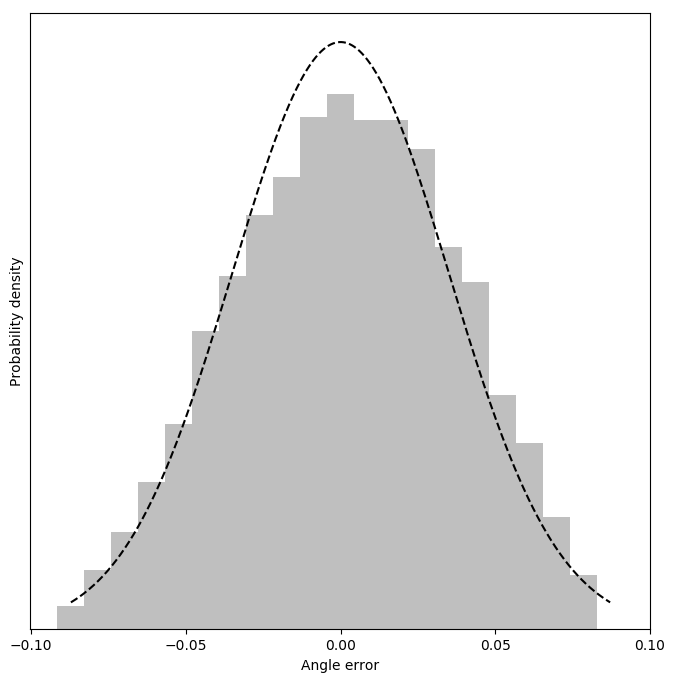
\includegraphics[width=\linewidth]{uncertainty}
  \end{minipage}
  \begin{minipage}{.5\textwidth}
    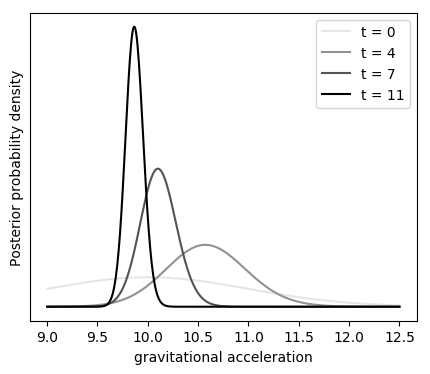
\includegraphics[width=0.97\linewidth]{posteriors}
  \end{minipage}
  \caption{Left: numerical forward propagation of time uncertainties through the pendulum model. Dashed line is the density function of the Gaussian used to model the uncertainty in the probabilistic model. Right: Sequence of posterior densities after observing $t=0, 3, 6, 9$ data points from light to dark, the lightest and darkest being respectively the prior and posterior density. }
  \label{uncertainty-posteriors}
\end{figure}


\begin{proof}
  We first prove that the solution $x(t)$ of the initial value problem is bounded, which is a stronger result than Assumption \ref{assumption-fw}(1). We start by defining the Hamiltonian
  \begin{equation*}
    H(x, x') = \frac12 x'^2 - \frac{g}{l}\cos(x).
  \end{equation*}
  By simple calculations, one can show that $H$ is constant along the solution of the initial value problem. Since the initial values are $x_0 \in (0, \pi/2)$ and $x_0' = 0$, we have $H(x(t), x'(t)) = -\frac{g}{l}\cos(x_0) \in (-\frac{g}{l}, 0)$ for all $t > 0$. Assuming that $x(t)$ is not bounded, since $x$ is continuous and $x_0 \le \pi/2$, there is a time $t^*$ such that $x(t^*) = \pi$, giving
  \begin{equation*}
    H(x(t^*), x'(t^*)) = \frac12 x'(t^*)^2 - \frac{g}{l}\cos(x(t^*)) \ge -\frac{g}{l}\cos(\pi) = \frac{g}{l} > 0.
  \end{equation*}
  This contradicts $H(x(t), x'(t)) = H(x_0, x'_0) \in (\frac{g}{l}, 0)$. Thus the solution of the initial value problem is bounded and so is $\mathcal{G}_t$ for every $t > 0$, proving i).
  Furthermore, we know that the solution of the initial value problem is continuously differentiable with respect to $g$, it is thus locally Lipschitz continuous everywhere, and so is $\mathcal{G}$, thus completing the proof.
\end{proof}

We have proven that the pendulum problem is well posed, and can now use the Bayesian solution to the inverse problem to estimate the true value of $g$ from our measurements of the system. The next chapter will study numerical approximation methods to estimate this solution.

%%% Local Variables:
%%% mode: latex
%%% TeX-master: "Thesis"
%%% End:
